\chapter{Il sistema climatico: componenti}
\section{Evidenze del Climate Change negli ultimi anni}
\begin{figure}[htpb]
    \centering
    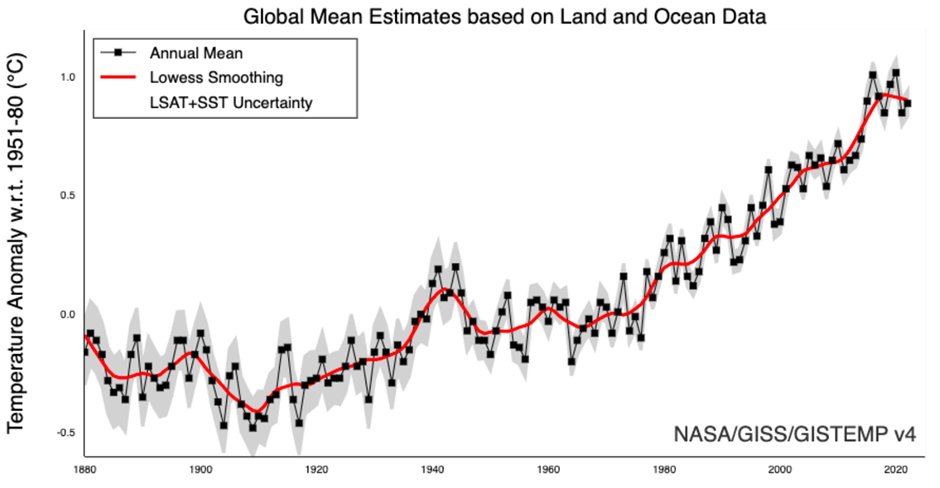
\includegraphics[width=0.5\linewidth]{uploads/CC.png}
\end{figure}
Rispetto ad un periodo di referenza come è cambiata la temperatura media. Nello studio del clima si studia l’anomalia: la differenza rispetto a una referenza, l’universo è scritto in differenze. 

H0 quando vediamo qualcosa che non funziona, che cambia l’assunzione è che è la natura, poi si possono ipotizzare vari altri motivi.

Statistica e significanza: dopo quante volte devo indovinare testa o croce affinché l’evento abbia significanza?
\begin{figure}[htpb]
    \centering
    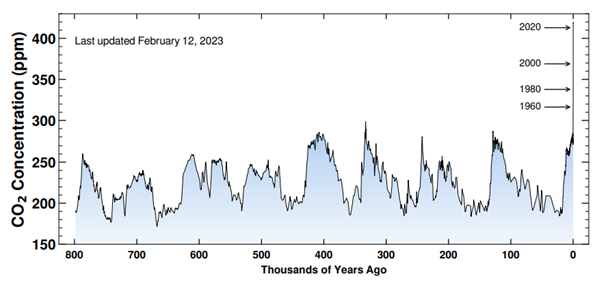
\includegraphics[width=0.5\linewidth]{uploads/CO2 concentration.png}
\end{figure}
\begin{figure}[htpb]
    \centering
    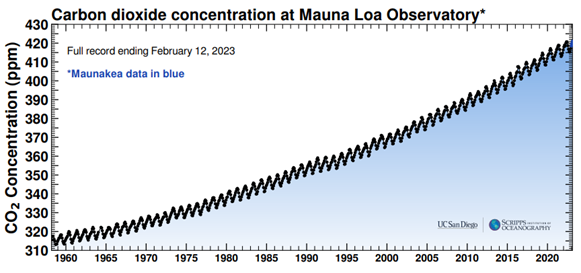
\includegraphics[width=0.5\linewidth]{uploads/manua loa.png}
    \caption{\href{http://keelingcurve.ucsd.edu }{Mauna Loa Data}}
\end{figure}
Humans are responsable perché si evidenziano dati di emissioni di combustibili fossili (facile trovare i dati), confrontando con l’incremento della CO2 sembra palese la responsabilità. 

\begin{figure}
    \centering
    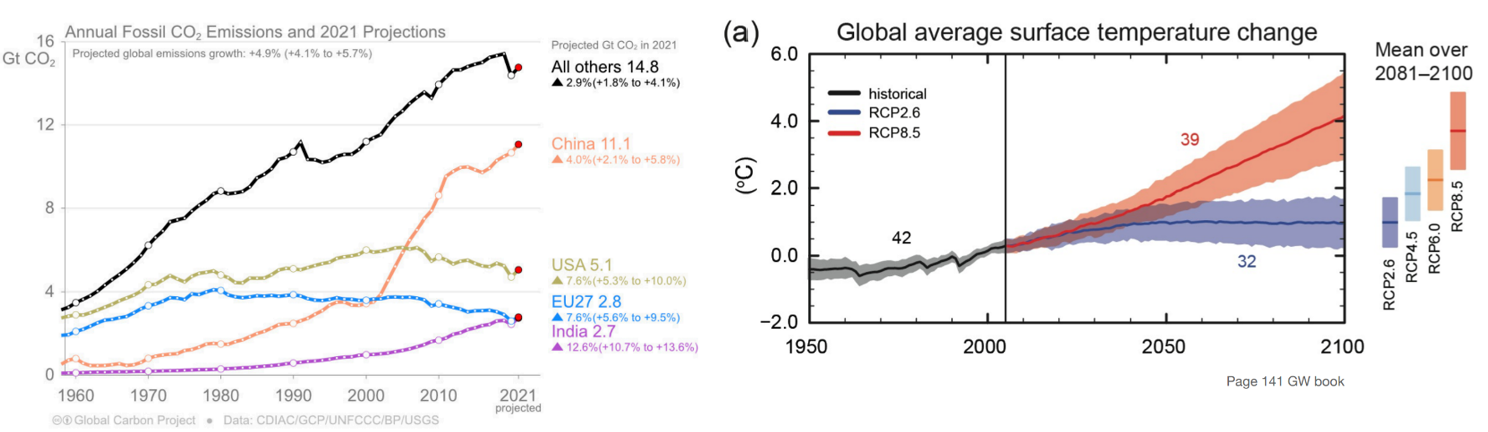
\includegraphics[width=0.85\linewidth]{uploads/aumento nel futuro.png}
    \caption{Aumento nel futuro}
\end{figure}
Clima è la statistica del tempo atmosferico. 

\section{Circolazione atmosferica}
L’energia che arriva ai tropici è più forte di quella che arriva ai poli. Ai poli la Terra emette più di quello che riceve: necessariamente parte dell’energia ai tropici arriva ai poli (energy transport) à la circolazione in atmosfera deve esserci. La circolazione atmosferica è forzata dalla differenza di ricezione di intensità luminosa. 

\begin{figure}[htpb]
    \centering
    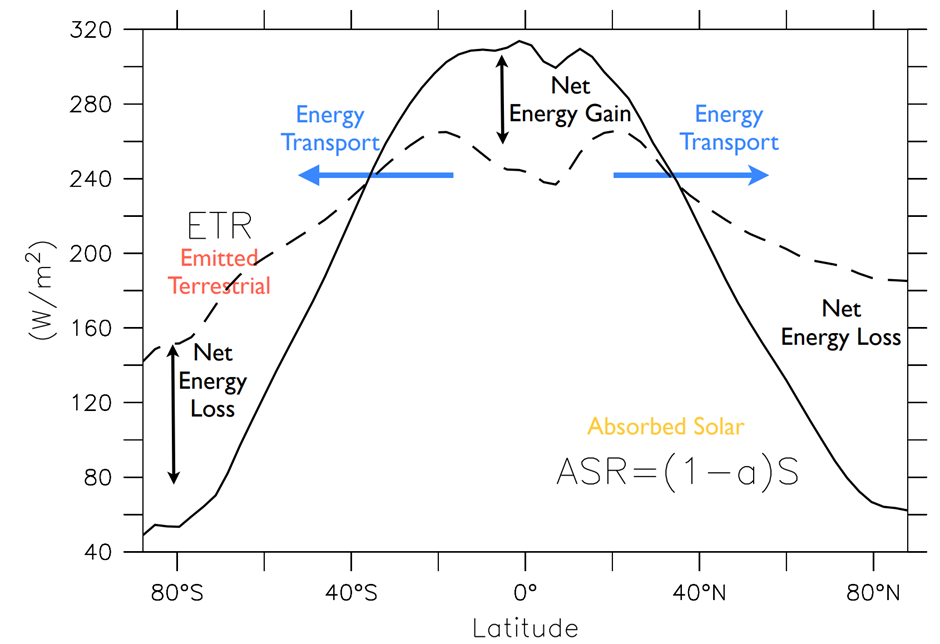
\includegraphics[width=0.5\linewidth]{uploads/heat trans.png}
\end{figure}

$900 W/m2$ a giugno.
La circolazione terrestre permette l'emissione di energia (più di quella che si ha in un pianeta senza atm e oceano) ai poli.
\subsection{Convezione}
Ai Tropici celle convettive, perturbazioni locali che si muovono molto poco. Extra tropici si muovono molto di più. Nell'oceano la variazione di pressione è lineare perché non è compresso, l'atmosfera sì.
\begin{figure}[htpb]
    \centering
    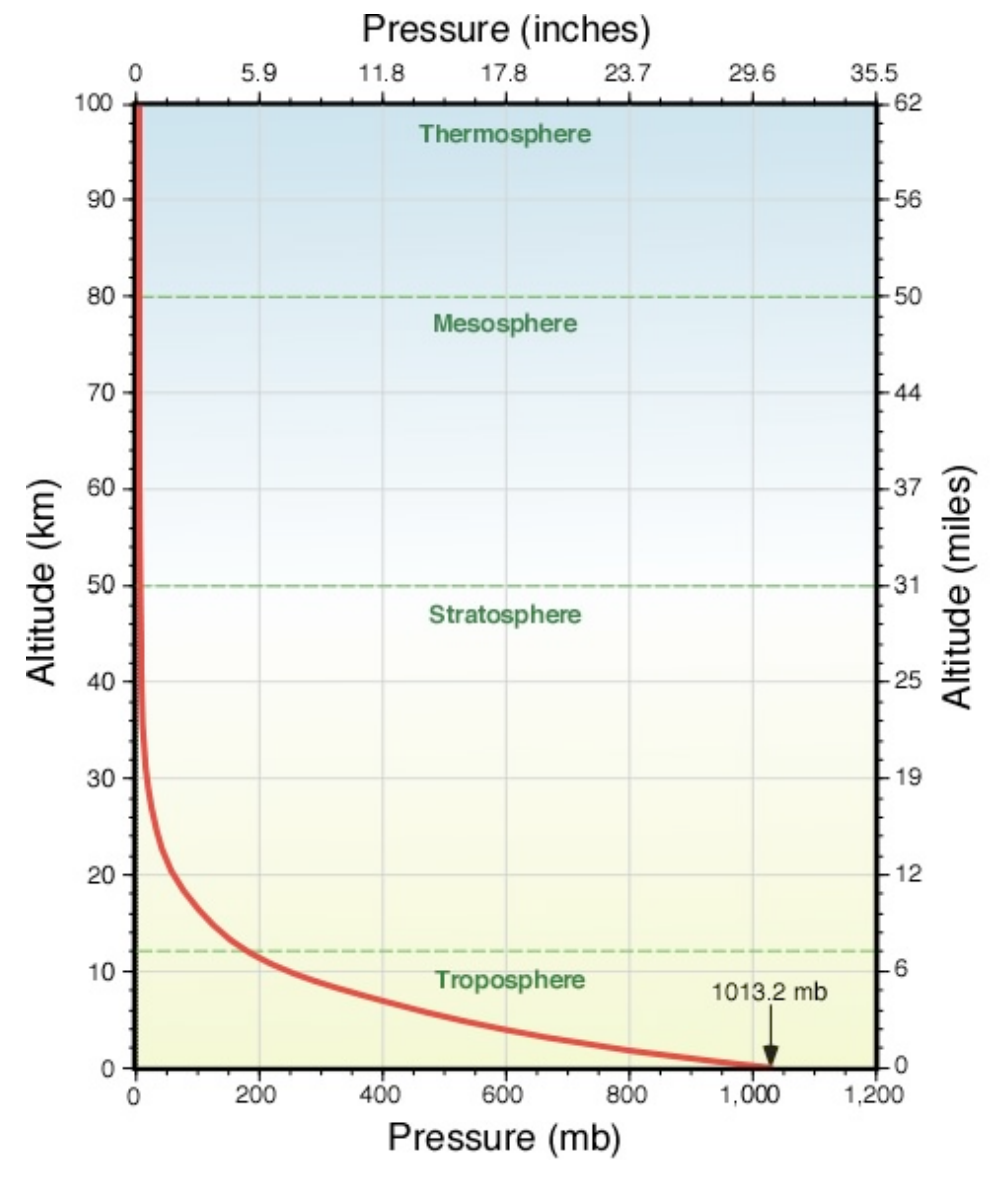
\includegraphics[width=0.35\linewidth]{uploads/pressure.png}
\end{figure}
La forza del vento è data dal gradiente di temperatura.
\begin{figure}[htpb]
    \centering
    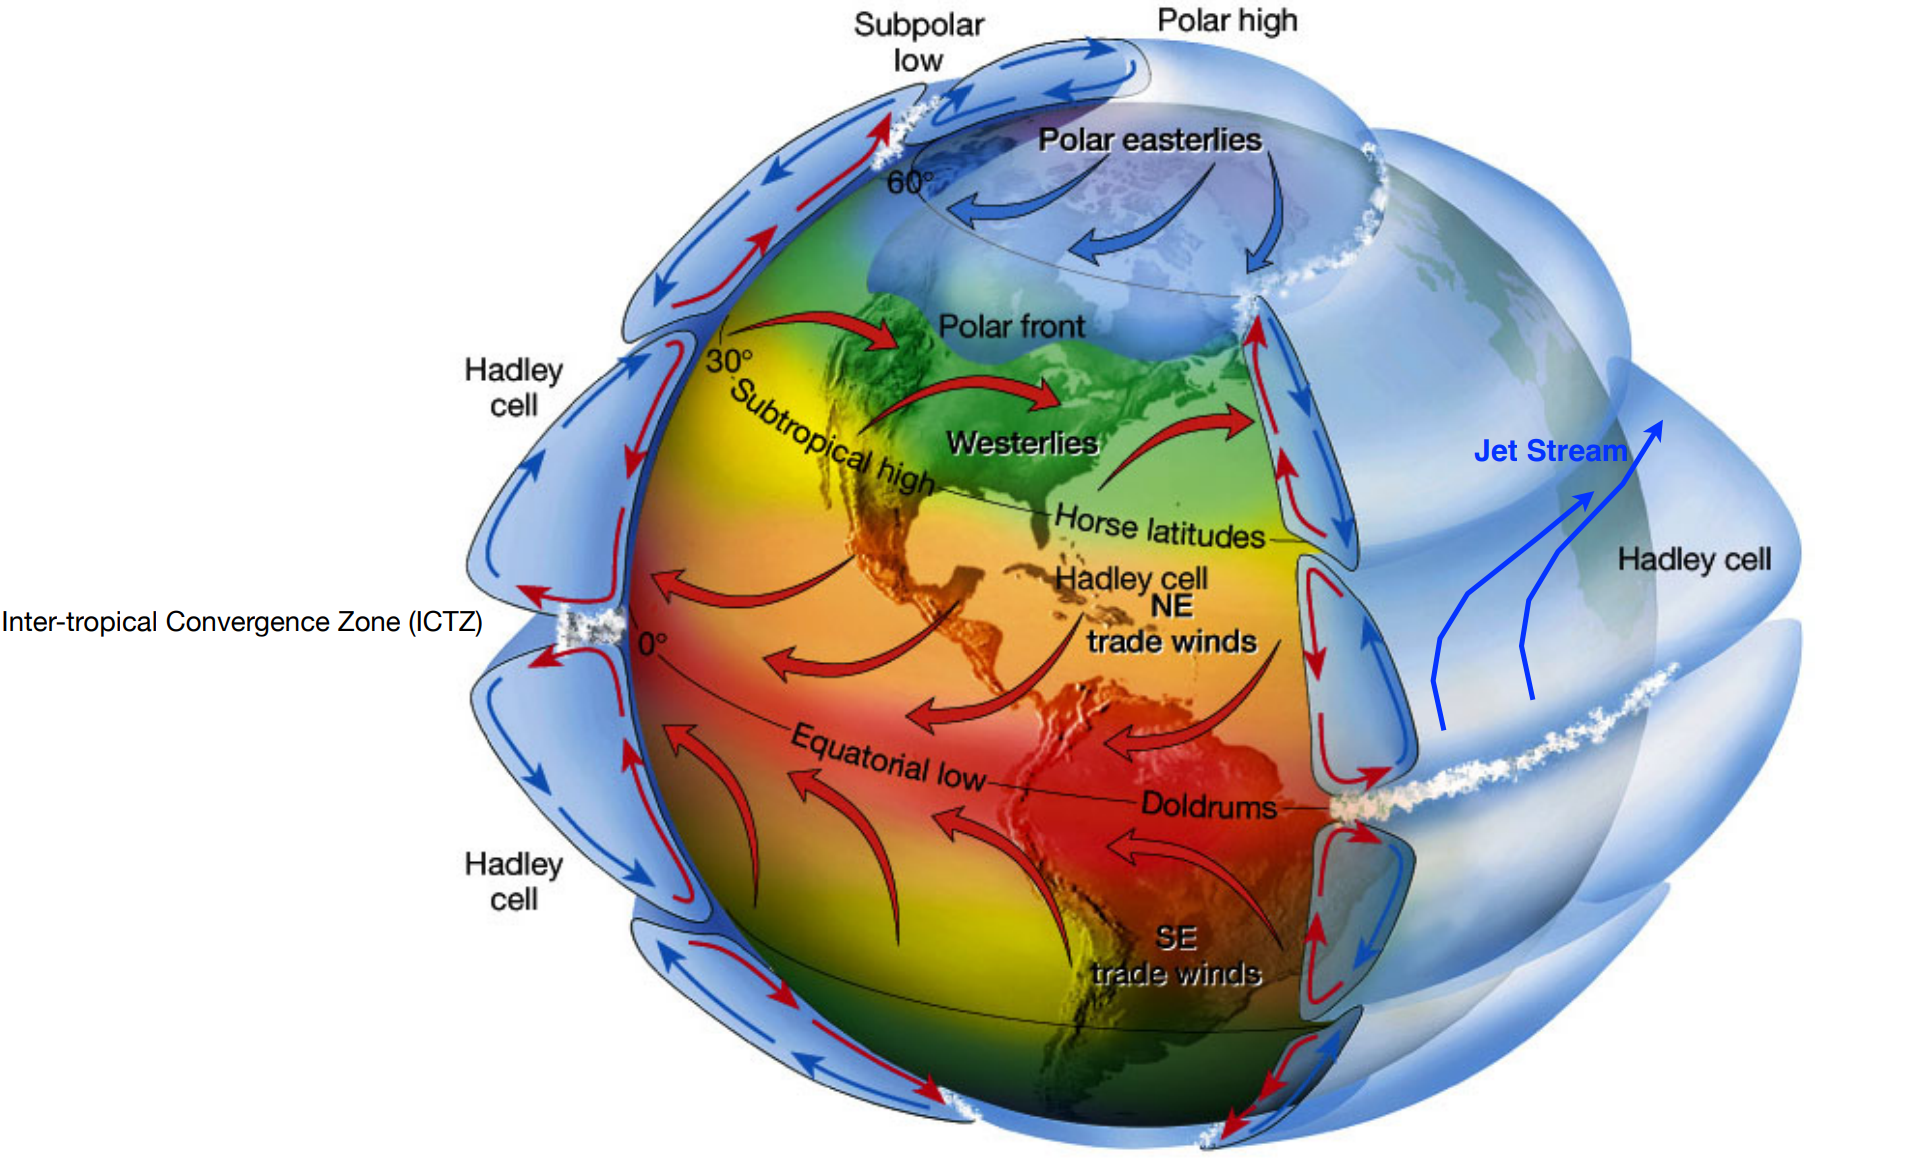
\includegraphics[width=0.5\linewidth]{uploads/modello a tre celle.png}
    \caption{Modello a tre celle}
    \label{fig:mod a tre celle}
\end{figure}
destra emisfero nord sx emisfero sud. Saturazione means 100\% di umidità. Umidità relativa: quanto vicino sei alla saturazione.

\begin{figure}[htpb]
    \centering
    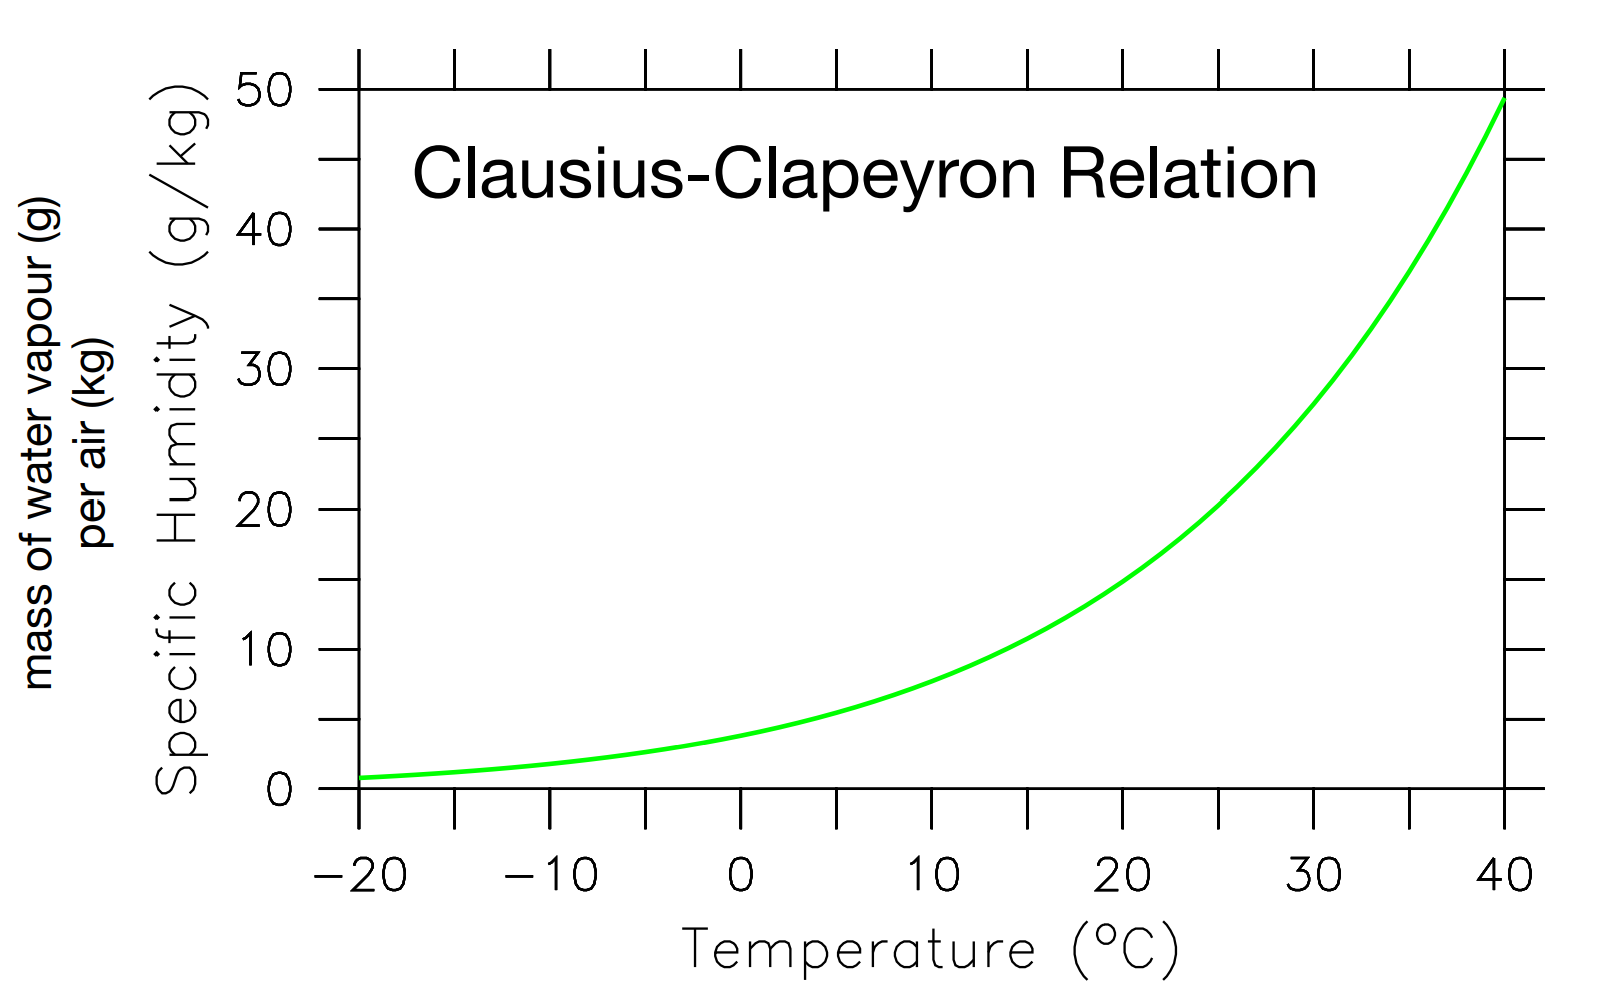
\includegraphics[width=0.5\linewidth]{uploads/CC equation.png}
\end{figure}

Riscaldando l'aria la saturazione diminuisce: sto dando più energia all'aria che riesce a mantenere in sospensione più molecole d'acqua $\rightarrow$ va giù la uminidtà relativa: la quantità d'acqua che c'è (ed è costante da prima e dopo) è più piccola di quella che ora l'aria può contenere NB se tu l'acqua non gliela dai se la prende da te (metti una scodella vicino al termosifone). 
Riscaldare il pianeta crea area più calda che può mantenere più acqua del 7\%, intensificando quindi precipitazioni più intense.


Cella di Hadley alle nostre lat: westerlies.

Pressione è un po' come dire densità dell'aria. salendo in altezza diminuisce la pressione. 
Per ogni kg d'aria ci sono 15g di acqua nel caso di saturazione. Estremi di precipitazione dovuti al climate change: ogni 1°C warming l'umidità aumenta del 7\%. Perché su fa più freddo? Perché l'aria è più fredda: $\Gamma_d=-6.5°C/km$ moist adiabatic lapse rate. pressione e densità per i gas sono praticamente la stessa cosa.  molto in alto p è più bassa, le molecole si devono allontanare. Le particelle d'aria salendo aumentano di volume. Teoria cinetica della temperatura: la temperatura sono le vibrazioni delle molecole dentro a un gas. Se l'aria è secca la temperatura va giù con $\Gamma_d=-10°C/km$. Se mi raffreddo l'umidità che posso contenere è molto più bassa (Clausius-Clapeyron) quindi le mol condensano. 

NB per far salire l'aria potrebbe esserci un fronte d'aria che spinge in alto altra aria calda. In eq la sup è molto calda, l'aria tende a salire poi nuvole e precipitazione: celle convettive. Oppure l'aria sale per condizioni orografiche. Se raffreddi l'aria questa inizia a condensare: spugna che si stringe.


Alcuni oggetti trattengono il calore meglio di altri perché l'acqua assorbe un sacco di calore, questa abilità di trattenere il calore è desritta dalla capacità termica. Legato a questo concetto è il ciclo stagionale: l'acqua ha una capacità termica molto alta: è difficile cambiarle temperature, tende ad essere molto stabile: vicino al mare il clima è più mite.
\begin{figure}[htpb]
    \centering
    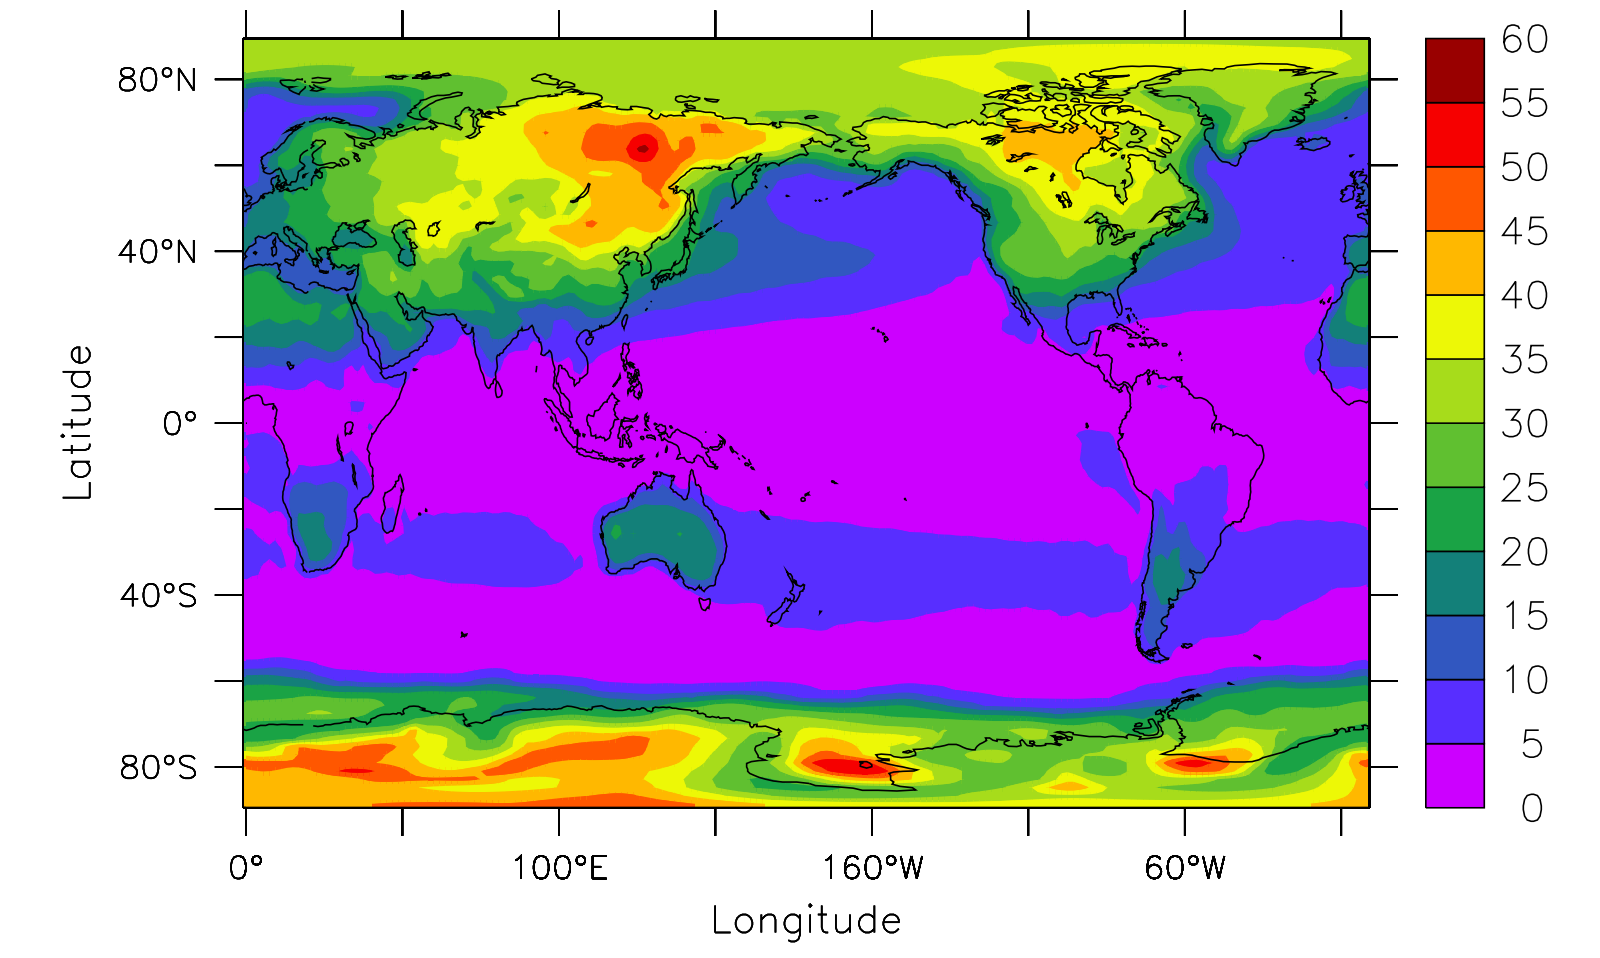
\includegraphics[width=0.5\linewidth]{uploads/Seasonal Cycle.png}
    \caption{Amplitude of Seasonal Cycle of Surface Air Temperatures. Large heat capacity of ocean dumps temperature variations.}
\end{figure}
earth nullschool
stat24


La circolazione poi complica le cose, anche per una previsione futura. Ad es Gulf stream porta energia e calore su.
\begin{figure}[htpb]
    \centering
    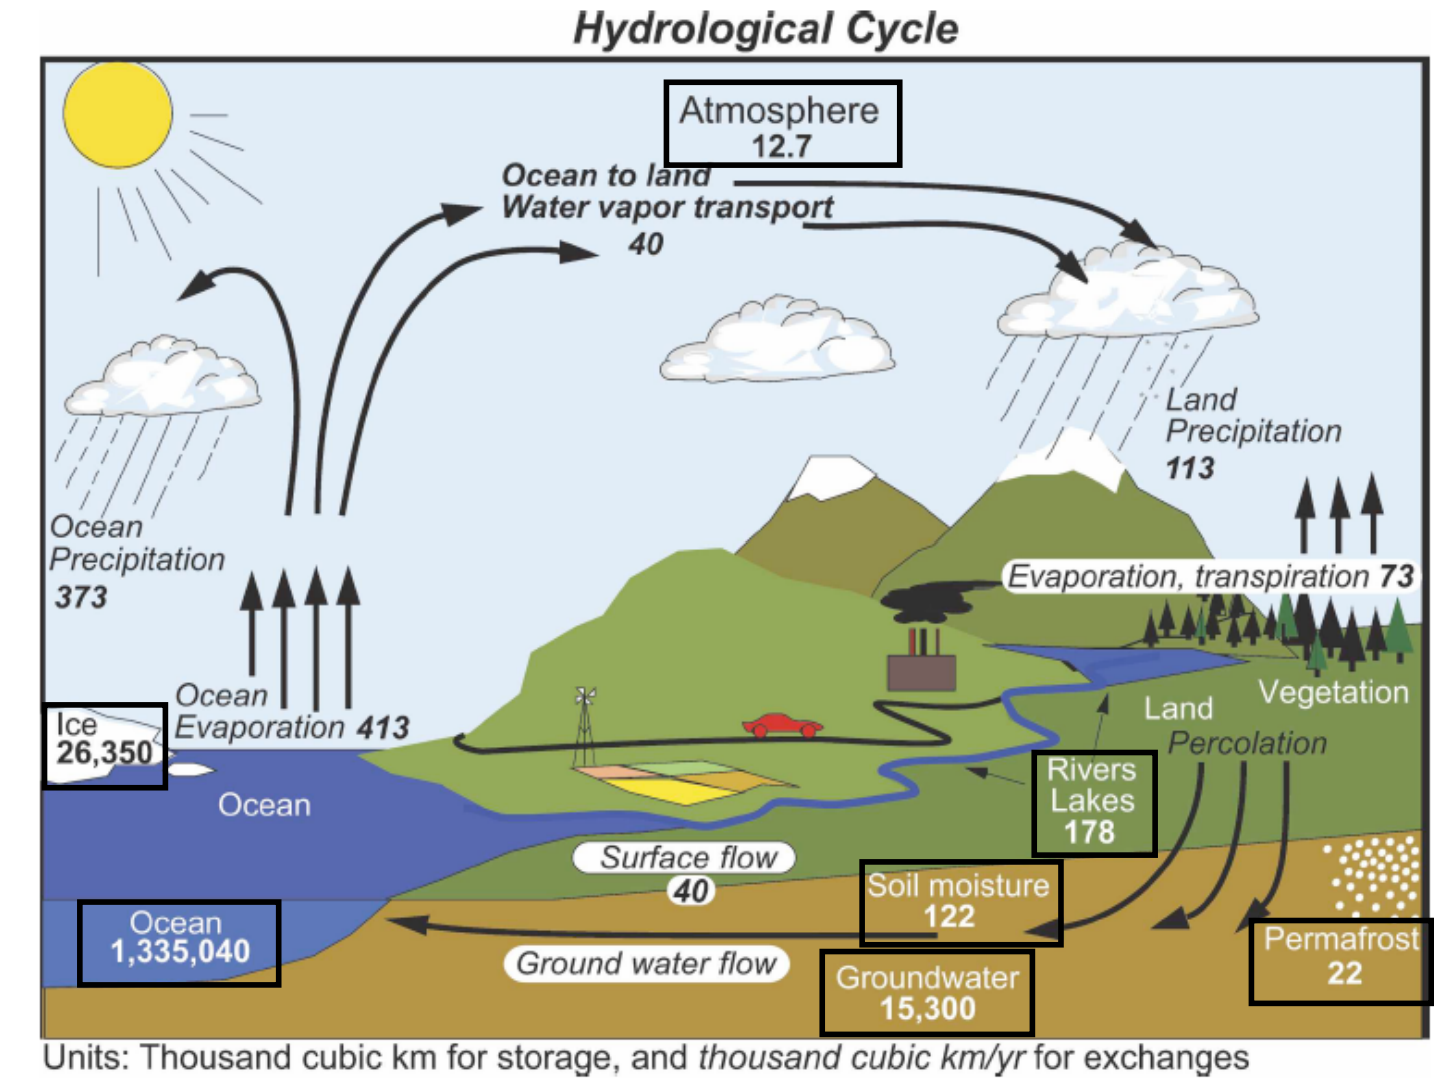
\includegraphics[width=0.5\linewidth]{uploads/hydro cycle.png}
\end{figure}
Che cosa accelera il ciclo idrologico?
\begin{itemize}
    \item Più evaporazione
    \item più trasporto di water vapor
    \item Più precipitation
\end{itemize}
Avere T più alta vuol dire che l'acqua evapora di più.

Quando fa molto freddo l'aria può trattenere meno vapore acqueo: vedo il fumo del respiro.
\section{Ocean Circulation}
Divisa in surface circulation and deep water circulation. In superficie l'acqua si muove perché spinta dal vento.
\begin{figure}[htpb]
    \centering
    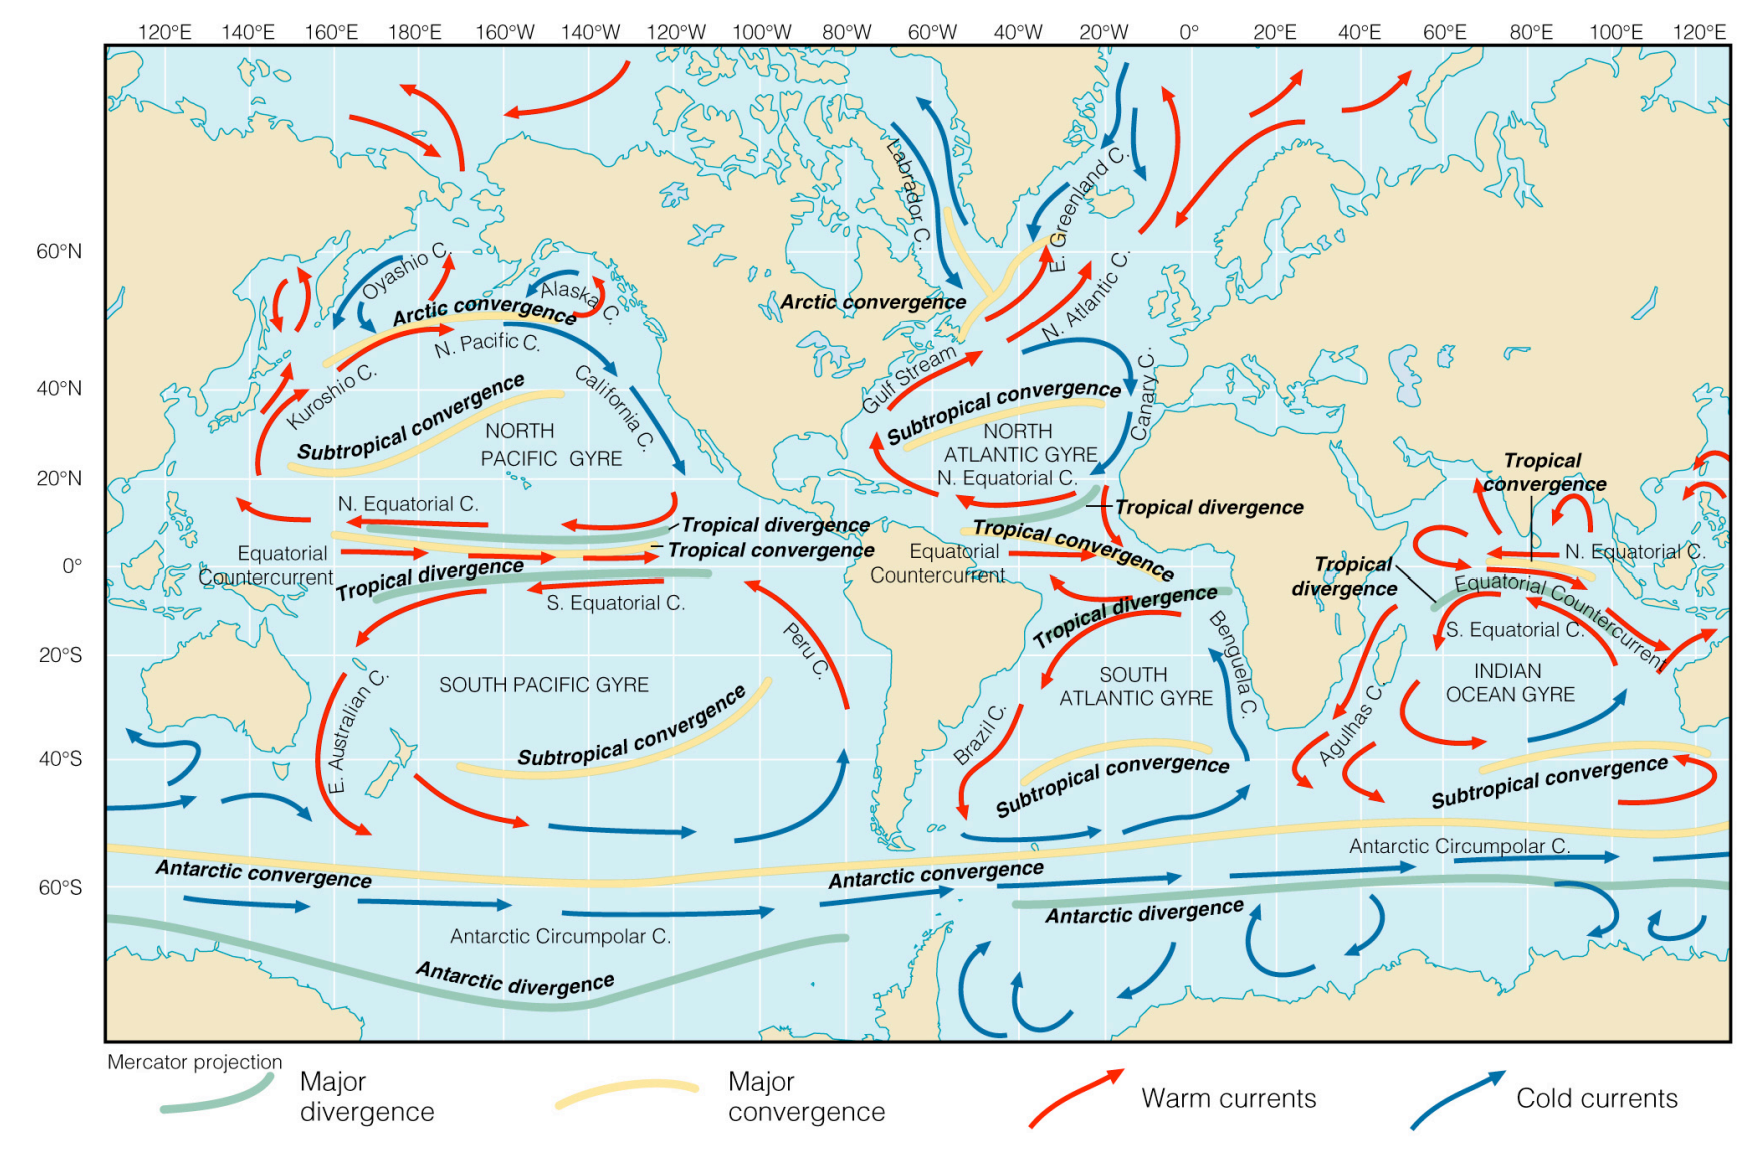
\includegraphics[width=0.5\linewidth]{uploads/Sea surface circulation.png}
    \caption{Sea surface circulation}
\end{figure}
\paragraph{Stratification}
Temperatura e salinità cambiano molto in profondità del mare: acqua superficiale è meno densa perché altrimenti sprofonderebbe: zone di generazione di acqua profonda vicino ai poli. 


Vento superficiale genera mixing in superficie: mix di temperature. Quando un fluido è vicino a un bordo si creano turbulenze per l'attrito: boundary layers. Correnti di marea (attrazione gravitazionale) agiscono su tutta la colonna d'aria, ci sono poi altre correnti associate alla global deep water circulation driven by temperature and salinity (density). Il bottom flow si forma in Antartide: Ross Sea and Weddell Sea. Nel Labrador Sea e Greenland Sea si forma acqua densa deep water. Quando fa freddo l'acqua è più densa. Le salinità nel Pacifico sono èiù basse, maggiore salinità maggiore densità.
\begin{figure}[htpb]
    \centering
    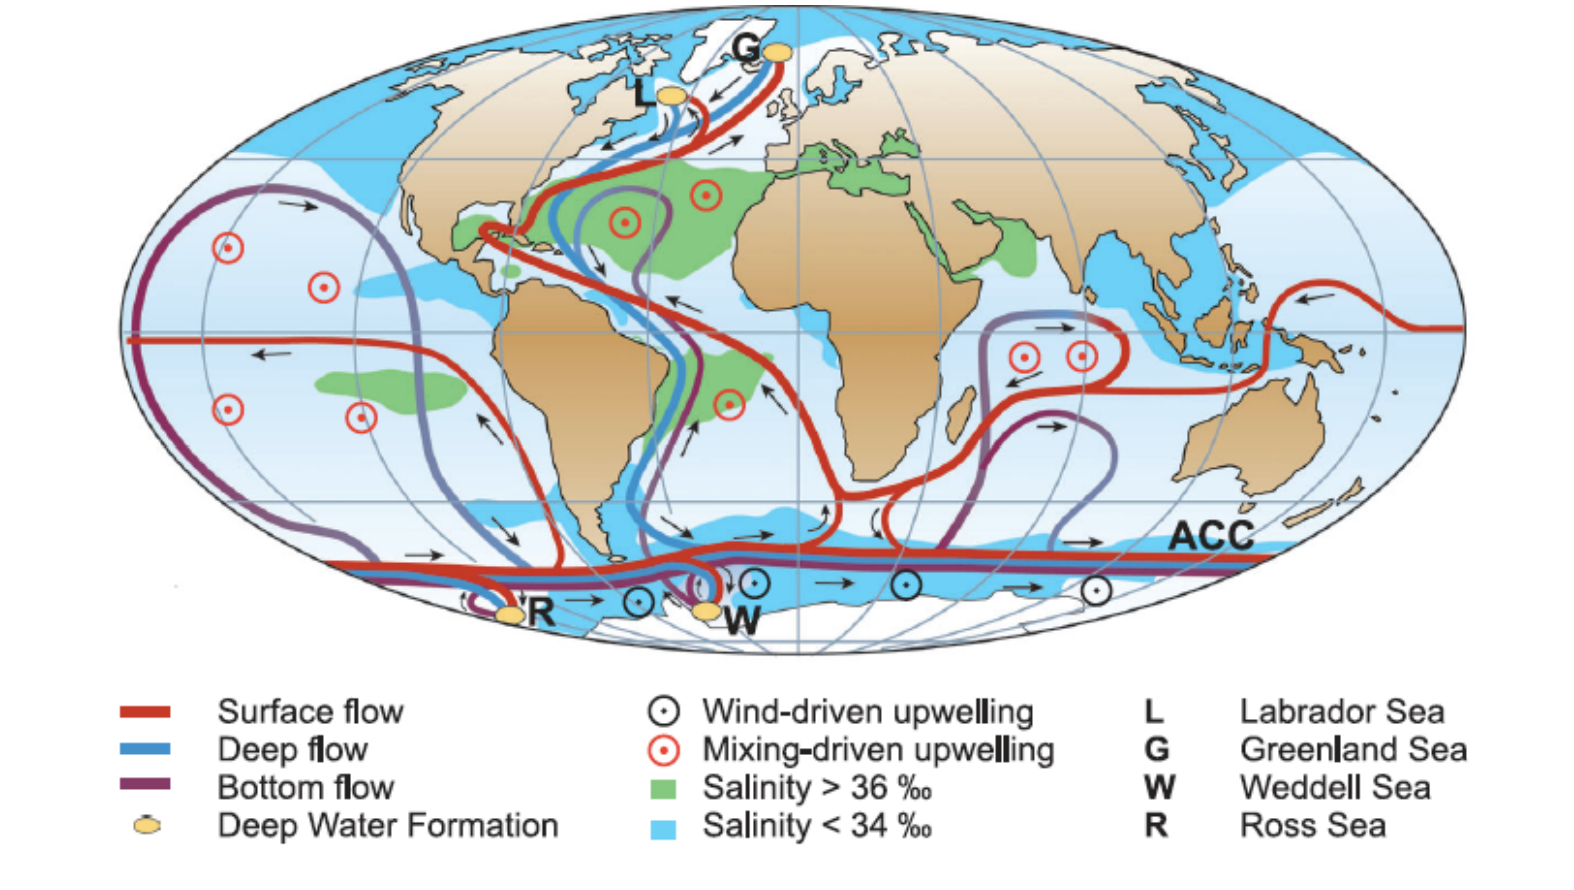
\includegraphics[width=0.5\linewidth]{uploads/global deep.png}
    \caption{Global Deep water circulation}
    \label{fig:deep water}
\end{figure}
\href{https://nsidc.org/home}{National snow and ice data center}

Antartica si forma molto sea ice: quando il mare ghiaccia il sale si deposita sotto: formazione di ghiaccio vuol dire più salinità nel mare: più densità: formazione di deep water. La chiamano anche Converior belt, Meridional overturning circulation, thermohaline, global deep water circulation.
\section{Criosfera} In cui l'acqua è allo stato solido, Aumenta albedo, si raffredda di più, si possono formare più ghiacci: feedback positivo.3
\begin{figure}[htpb]
    \centering
    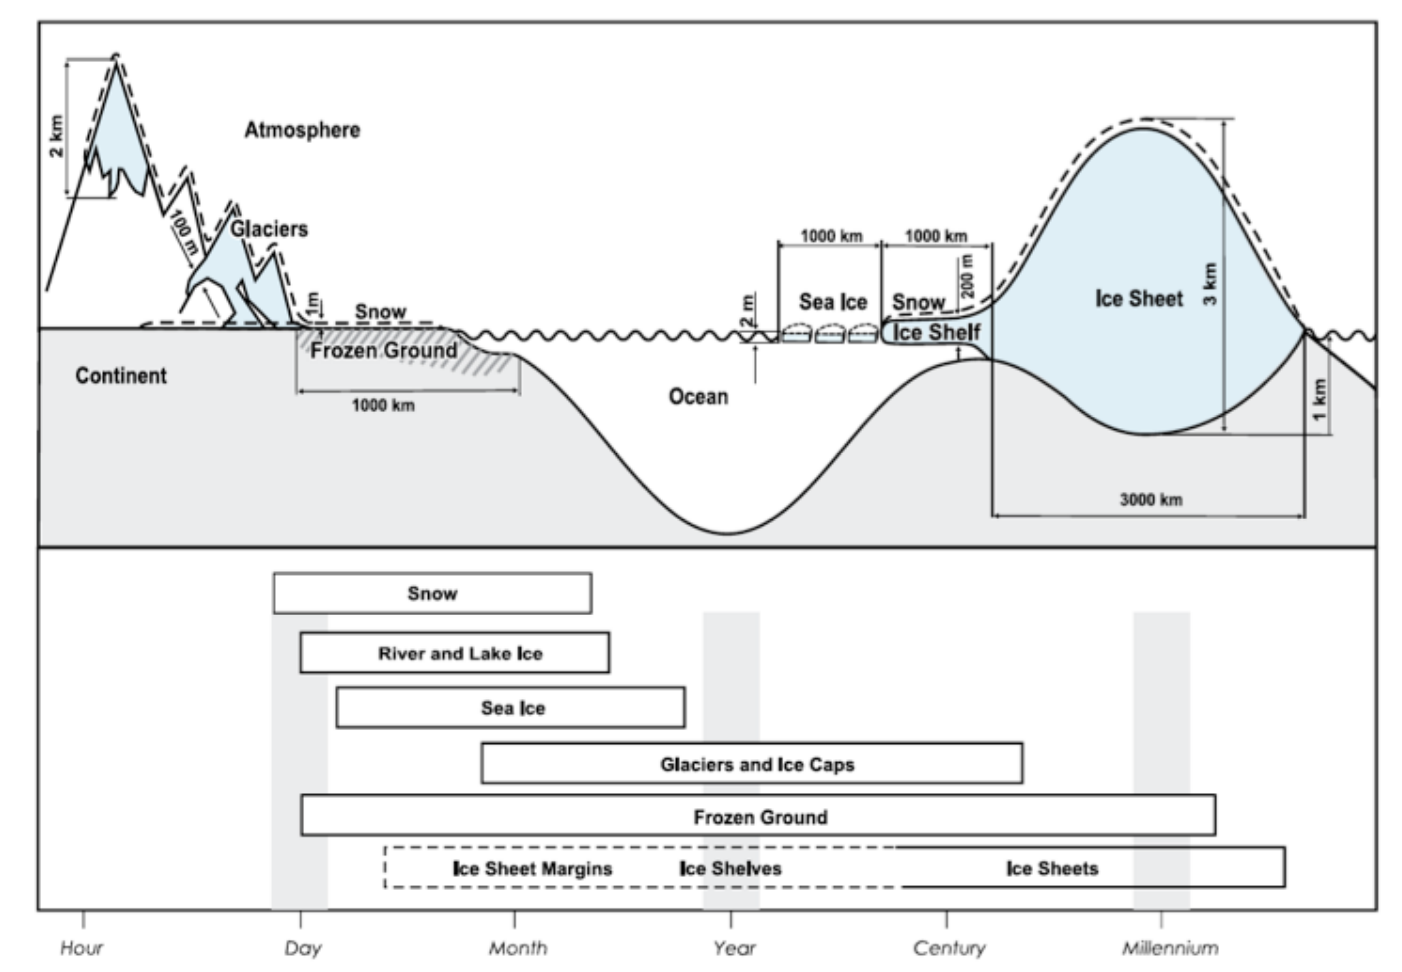
\includegraphics[width=0.5\linewidth]{uploads/criosfera.png}
    \caption{Components of the cryosphere}
    \label{fig:criosfera}
\end{figure}
Riserve più grossi come l'Antartica o la Groenlandia avrebbero più effetti sul sea level rise. Ghiaccio che galleggia non contribuisce al sea level rise: Spinta di Archimede, occupa il volume del liquido spostato.
\begin{figure}
    \centering
    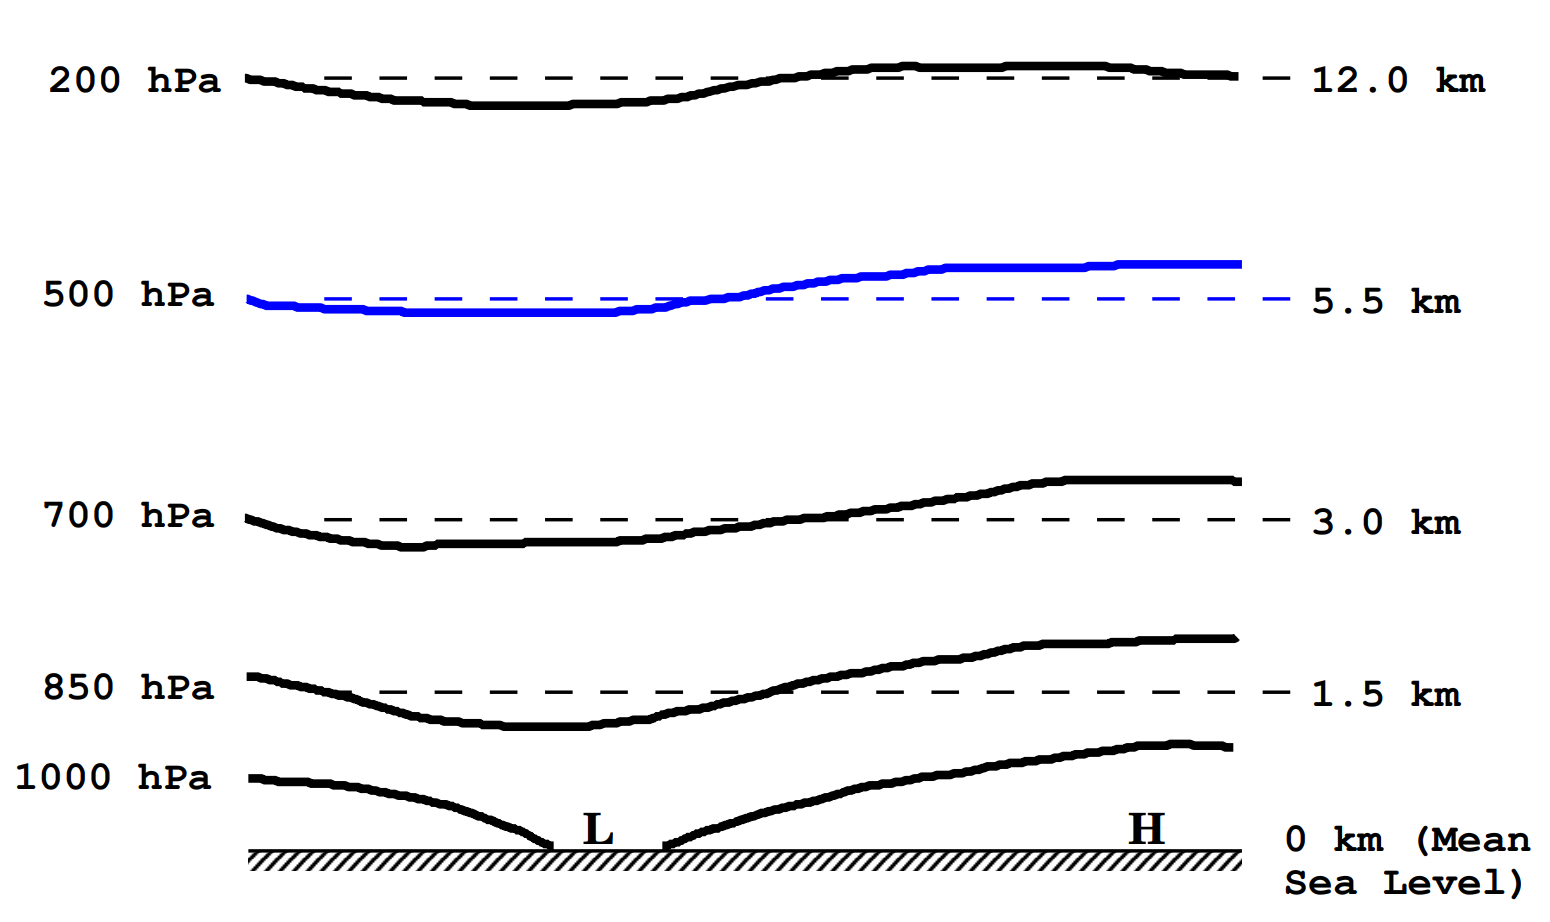
\includegraphics[width=0.5\linewidth]{uploads/hPa.png}
    \caption{hPa}
\end{figure}